% arara: xelatex: { shell : yes }
% arara: xelatex: { shell : yes }
% arara: xelatex: { shell : yes }

% kompilace xelatex prezentace.tex
% dokumentace k beameru: http://ftp.cvut.cz/tex-archive/macros/latex/contrib/beamer/doc/beameruserguide.pdf

% nastavení formátu prezentace 16:9 
\documentclass[czech,aspectratio=169]{beamer}

\usepackage{polyglossia}
\setmainlanguage{czech}

% nastavení vzhledu 
% další možnosti vzhledu viz https://hartwork.org/beamer-theme-matrix/
\usetheme{Madrid}
\usecolortheme{whale}

% vzhled slajdů vnitřní téma (např. vzhled odrážek)
\useinnertheme{rectangles} %možnosti: default circles rectangles rounded inmargin
% vzhled slajdů vnější téma
\useoutertheme{default} %možnosti: default, miniframes, smoothbars, sidebar, split, shadow, tree, smoothtree, infolines

% zavedeme čvutí modou barvu
\definecolor{CVUT}{HTML}{0065BD}
% čvutí modou použijeme jako hlavní barvu prezentace
\setbeamercolor{structure}{bg=white,fg=CVUT}

% jako font prezentace nadefinujeme oficiální ČVUT písmo Technika -- pokud chcete použít, musíte si font nainstalovat nebo jej nahrát na Overleaf
% https://www.cvut.cz/logo-a-graficky-manual  -- inforek, přihlášení přes celoškolské heslo
%\usepackage{fontspec}
%\setsansfont{Technika-Kniha}

% vypneme navigační panel beamer (pro zapnutí zakomentujeme)
%\beamertemplatenavigationsymbolsempty

% vygenerujeme slajdy s poznámkami -- ty si můžete vytisknout a mít je na obhajobu s sebou (pokud zapomenete slova, nebo kdyby nefungovalo promítání z nějakého důvodu)
%\setbeameroption{show notes}

% další balíčky
\usepackage{graphicx}
\usepackage{minted}
\usepackage{hyperref}
\usepackage{tikz}
\usetikzlibrary{chains,fit,shapes}

% Údaje o prezentaci
\title[Kooperativní mobilní multiplatformní hra]{Kooperativní mobilní multiplatformní hra}
\subtitle{Bakalářská práce}
\institute[FIT ČVUT v Praze]{Fakulta informačních technologií \\ České vysoké učení technické v Praze}
\author[J. Bittner]{Jan Bittner \\ Vedoucí práce: Ing. Marek Suchánek}
\date{5. 5. 2020}
\titlegraphic{
\includegraphics[width=.1\textwidth]{slides/logo-cvut}}

\begin{document}
  \begin{frame}
    \titlepage 
    \note{Nezapomenout pozdravit} %tohle je poznámka, ta na slajdu nebude, ale vygeneruje se vedle něj, pokud odkomentujete příkaz výše -- \setbeameroption{show notes} 
  \end{frame}
  
  %\begin{frame}
  %  \tableofcontents %generuje se automaticky z section, subsection, subsubsection
  %\end{frame}
  
  \begin{frame}{Cíle práce}
    \begin{itemize}
      \item analýza podobných aplikací a trendů
      \item analýza technologií pro vývoj
      \item návrh hry a herní logiky
      \item návrh a implementace hry
      \item otestování funkčnosti
    \end{itemize}
  \end{frame}

  \begin{frame}{Motivace}
    \begin{itemize}
      \item 77 \% uživatelů mobilních zařízeních jsou hráči.
      \item Framework Flutter je nový. (todo: a proto je skvělé objevit jeho limity)
      \item Obohacení Flutter komunity. (todo) 
      \item Vytvoření open-source hry. (otevřená možnost; mohou využít začínající vývojáři etc.)
    \end{itemize}
  \end{frame}

  \begin{frame}{Technologie}
    \begin{columns}
      \begin{column}{.33\textwidth}
        \begin{center}
          \textbf{Flutter}

          Multiplatformní mobilní framework
        \end{center}
      \end{column}
      \begin{column}{.33\textwidth}
        \begin{center}
          \textbf{Bloc}

          Knihovna pro state management
        \end{center}
      \end{column}
      \begin{column}{.33\textwidth}
        \begin{center}
          \textbf{Clean Architecture}

          Architektura
        \end{center}
      \end{column}
    \end{columns}
  \end{frame}

  \begin{frame}
      \begin{center}
        {\large ``The way you keep software soft is
      to leave as many options open as possible,
      for as long as possible.
      What are the options that we need to leave open?\\
      They are the details
      that don’t matter.''}
      \vskip5mm
      --- Robert C. Martin, Clean Architecture
      \end{center}
  \end{frame}

  \begin{frame}
    \begin{center}
      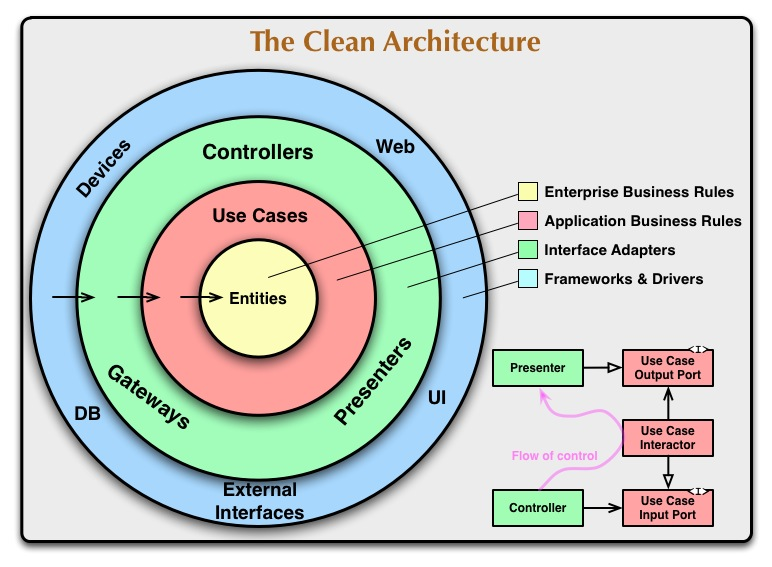
\includegraphics[width=.6\textwidth]{slides/logo-clean-architecture}
    \end{center}
  \end{frame}

  \begin{frame}{Návrh hry}
    % TODO: diagram jeden hráč aktér, druhý manuál
    % TODO: nějaký diagram event loop
  \end{frame}

  \begin{frame}{Návrh hry}

  \end{frame}

  \begin{frame}
    \begin{columns}
      \begin{column}{.33\textwidth}
        \begin{center}
          Screen 1
        \end{center}
      \end{column}
      \begin{column}{.33\textwidth}
        \begin{center}
          Screen 2
        \end{center}
      \end{column}
      \begin{column}{.33\textwidth}
        \begin{center}
          Screen 3
        \end{center}
      \end{column}
    \end{columns}
  \end{frame}

  \begin{frame}{Shrnutí}
    \begin{itemize}
      \item Rešerše technologií.
      \item Vytvoření funkčního řešení hry.
      \item Možnosti rozšíření.
      \item ---
      \item TODO: osobní přínosy -- naučení se technologií, obohacení komunity o hru ve Flutteru, možnost na volné chvilky s přáteli...
    \end{itemize}
  \end{frame}

  \begin{frame}[noframenumbering]{Otázky oponenta}
    Otázka první: Proč?

    \vfill

    Odpověď: Prostě proto.
  \end{frame}

  \begin{frame}[noframenumbering]{Otázky oponenta}
    Otázka druhá: Proč?

    \vfill

    Odpověď: Prostě proto.
  \end{frame}
\end{document}

% TODO...
% clean architecture citát - strana
% clean architecture obrázek https://blog.cleancoder.com/uncle-bob/2012/08/13/the-clean-architecture.html
% fakta z motivace -- wepc_video_game_statistics
